\leftsection{Технологическая часть}
В данном разделе будут рассмотрены реализации алгоритмов визуализации и
средства их реализации.

\subsection{Средства реализации}
Для реализации алгоритмов в данной работе был выбран язык C++, так как
данный язык предоставляет возможность решить поставленную задачу и реализовать
объектно-ориентированную модель для построения модифицируемой системы.
В качестве компилятора для программы используется GNU GCC.

\subsection{Диаграмма классов}
На рисунке \ref{fig:uml_diag} предсавлена диаграмма классов разработанного
приложения.

\clearpage

\begin{sidewaysfigure}[!h]
    \centering
    \def\svgwidth{\textheight}
    \input{uml_diag.pdf_tex}
    \caption{Диаграмма классов}
    \label{fig:uml_diag}
\end{sidewaysfigure}

\clearpage

\subsection{Сведения о модулях программы}
Программа состоит из следующих модулей:
\begin{itemize}
    \item \verb|scattering_propoerties/*| --- свойства (аргументы) функций рассеивания;
    \item \verb|boundings/*| --- объемлющие оболочки геметрицеских объектов;
    \item \verb|display_transform_strategies/*| --- стратегии преобразования изображения в расширенном динамическом пространстве;
    \item \verb|light_tracers/*| --- трассировщики источников света;
    \item \verb|material_properties/*| --- свойства материлов;
    \item \verb|math/*| --- математические абстракции (точка, вектор, нормаль, луч, преобразования);
    \item \verb|matrix/*| --- реализация матрицы;
    \item \verb|projections/*| --- проекции из пространства камеры в глобальные координаты;
    \item \verb|renderers/*| --- визуализаторы;
    \item \verb|scattering_builders/*| --- строители функций рассеивания;
    \item \verb|scattering_functions/*| --- функции рассеивания;
    \item \verb|scene_tracers/*| --- трассировщики сцены;
    \item \verb|shapes/*| --- геометрические объекты;
    \item \verb|shape_builders/*| --- строители геометрических объектов;
    \item \verb|shape_properties/*| --- свойства геометрических объектов;
    \item \verb|shape_properties/projectors/*| --- виды камер;
    \item \verb|shape_samplers/*| --- 
    \item \verb|shape_tracers/*| --- трвссировщики геометрических объетов;
    \item \verb|texture/*| --- текстуры;
    \item \verb|texture_builders/*| --- строители текстур;
    \item \verb|texture_mappers/*| --- преобразователи текстурных координат;
    \item \verb|tracers/*| --- трассировщики путей;
    \item \verb|tracer_builders/*| --- строители трассировщиков путей;
    \item \verb|tracer_properties/*| --- свойства (аргументы) трассировщика путей;
    \item \verb|intersection| --- пересечение луча с геометрическим объектом;
    \item \verb|scattering_unit| --- модуль рассеивания;
    \item \verb|tracer_info| --- коллекция свойст трассировщика;
    \item \verb|hdr_display_linker| --- модуль связи адаптеров дисплея расширенного динамического диапазона;
    \item \verb|material| --- материал, коллекция свойств материалов;
    \item \verb|scene| --- сцена, коллекия геометрических объектов и их свойств;
    \item \verb|tracing_unit| -- модуль, представляющий  взаимодействия на границе сред;
    \item \verb|intensity| --- интенсивность;
    \item \verb|scattering_info| --- коллекция свойств функций рассеивания;
    \item \verb|tools| --- модуль, содержащий прикладные функциии;
    \item \verb|transform_strategies| --- стратегии преобразования геометрических объектов.
\end{itemize}

\subsection{Реализации алгоритмов}
На листингах \ref{code_complete_renderer-h} -- \ref{code_complete_tracer-cpp},
\ref{code_complete_tracer-h} -- \ref{code_complete_tracer-cpp}
представлена реализация классов, отвечающих за алгоритм трассировки путей, и
вычисления функций рассеивания, а на листингах \ref{code_direct_lighting}
и \ref{code_sampling_lighting} --- реализация алгоритмов вычисления освещенности
в точке.

\lstinputlisting[language=c++, label={code_complete_renderer-h}, caption={Листинг кода визуализатора в алогритме трассировки путей (1)}]{../../inc/renderers/complete_renderer.h}
\lstinputlisting[language=c++, label={code_complete_renderer-cpp}, caption={Листинг кода визуализатора в алогритме трассировки путей (2)}]{../../src/renderers/complete_renderer.cpp}
\lstinputlisting[language=c++, label={code_complete_tracer-h}, caption={Листинг кода трассировщика в алогритме трассировки путей (1)}]{../../inc/tracers/complete_tracer.h}
\begin{lstlisting}[language=c++, label={code_complete_tracer-cpp}, caption={Листинг кода трассировщика в алогритме трассировки путей (2)}]
...
Intensity<> CompleteTracer::trace(const Scene &scene, const Ray3<double> &ray) const
{
    SimpleSceneTracer stracer;
    SamplingLightTracer ltracer (scene, this->light_samples);

    common_prop_t common = get_common_prop(scene);
    ScatteringUnit head (scene,
                         std::list<std::shared_ptr<const ScatteringFunction>>(),
                         ray);
    head.scatter(stracer);

    std::stack<stack_tracing_unit_t> stack;

    for (std::shared_ptr<TracingUnit> &unit : head)
        stack.push({unit, {}, 1, false});

    while (0 != stack.size())
    {
        stack_tracing_unit_t &current = stack.top();

        if (!current.start)
            init_unit_arg(common, scene, current, stracer, ltracer);
        else
            current.unit->accumulate(current.iter++);

        if (current.unit->isTerminate() || current.unit->end() == current.iter)
            stack.pop();
        else if (this->max_depth > current.depth)
            for (std::shared_ptr<TracingUnit> &unit : **current.iter)
                stack.push({unit, {}, current.depth + 1, false});
    }

    Intensity<> out;

    for (std::shared_ptr<TracingUnit> &unit : head)
        out += unit->getBaseIntensity() * unit->getEmission();

    return out;
}
...
\end{lstlisting}

\subsection{Интерфейс программы}

Интерфейс разработанного приложения приведен на рисунке~\ref{fig:interface}

\begin{figure}[h]
    \centering
    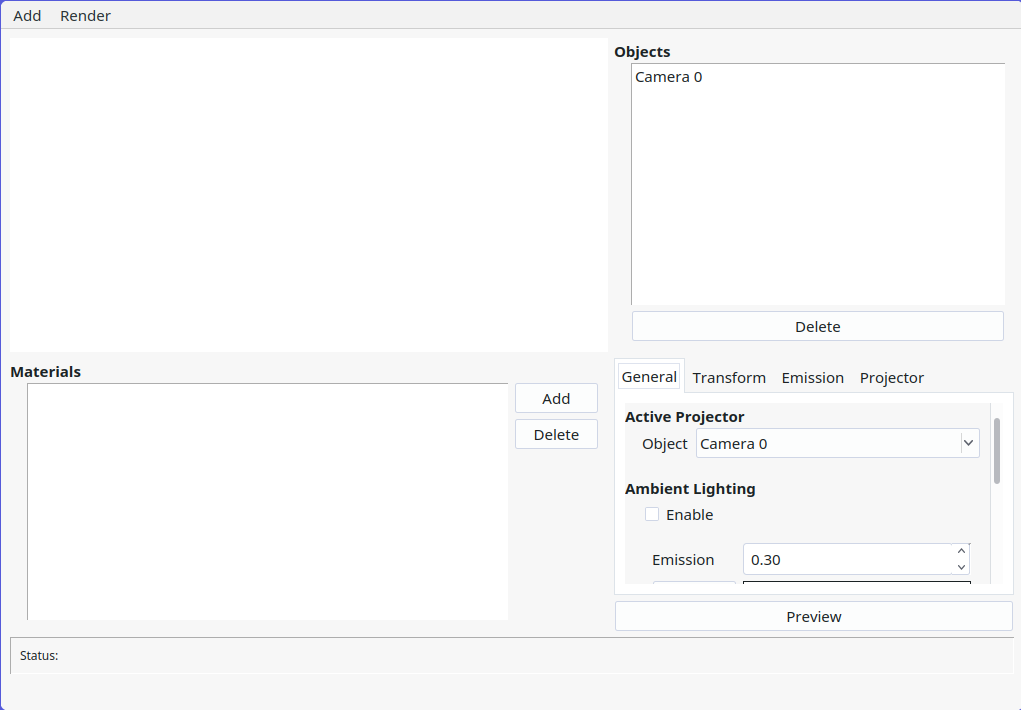
\includegraphics[width=0.9\textwidth]{image/demo/main.png}
    \caption{Интерфейс программы}
    \label{fig:interface}
\end{figure}

\subsection*{Вывод}
В данном разделе были рассмотрены реализации алгоритмов визуализации.

\pagebreak

